% Capítulo 9. Sensibilidad, incertidumbre y repetibilidad (rúbrica 40 pts).

\section{Qué parámetros se sensibilizan y por qué}
\label{sec:justificacion-sens}

Los parámetros se eligieron a partir de los supuestos de la Tabla~\ref{tab:supuestos} y de las preguntas que RED tendría que responder antes de adoptar el plan. Se agrupan en tres familias.

La primera es la capacidad de carga. Las plazas y conexiones son la infraestructura que RED puede ampliar o perder, y el límite eléctrico es un supuesto porque el dato del transformador no existe. Por eso se probaron plazas y conexiones con 20\,\% menos y con 20 y 50\,\% más, la mitad de las conexiones con las mismas plazas, el cierre de cada electroterminal por separado, que mide la resiliencia frente a una falla, y las plazas repartidas según las corridas de cada sector, a propósito del desbalance que preguntó el profesor. Junto con ellas se probó la tarifa de punta un 50\,\% más cara, para ver si el plan mueve su carga de horario.

La segunda es el bus. La batería y el consumo deciden cuántas corridas alcanza a hacer cada bus, y el consumo de \Consumo~kWh/km es un supuesto derivado de la autonomía nominal que ignora la pendiente, el clima y la carga de pasajeros. Se probaron baterías de 300 y 250~kWh, que representan buses distintos o baterías degradadas, y un consumo 10 y 20\,\% mayor.

La tercera son los precios. El costo por bus y por kilómetro vienen del enunciado y no necesariamente son costos reales, así que se variaron en 20\,\% hacia arriba y hacia abajo, y además se agregó el costo de espera que el modelo no cobra.

Cada escenario de capacidad, tarifa y bus se corrió con el plan inicial y con cuartetos al azar, una semilla y 20 minutos, y se compara con una base corrida en la misma tanda, en el mismo computador y con cuatro corridas en paralelo. Los escenarios de precios se evaluaron sobre los mismos planes, sin volver a optimizar. Como con 20 minutos las tres semillas de la base difieren en \RuidoSemillas\,\% de costo, un cambio menor a unos 0,15\,\% no se puede atribuir al escenario. El plan inicial no tiene azar y sirve para confirmar la dirección de cada efecto. %literal

\section{Capacidad de carga y tarifa}
\label{sec:sens-capacidad}

La Tabla~\ref{tab:sensibilidad} y la Figura~\ref{fig:sensibilidad} muestran el resultado. Lo único que mueve el costo es cerrar un electroterminal, y depende de cuál. Cerrar El Conquistador cambia la flota en \SensBusesCierreDos{} buses y el costo en \SensCostoCierreDos\,\%, y cerrar La Reina, en \SensBusesCierreCuatro{} buses y \SensCostoCierreCuatro\,\%. Cerrar Vespucio Norte tiene un efecto intermedio, y cerrar Santa Rosa o Los Espinos queda dentro del ruido. El plan inicial confirma el mismo orden. Aun en el peor cierre el aumento es menor a 1\,\%, porque los buses del sector afectado pueden cargar en otro electroterminal y, como casi no cargan durante el día, el desvío pesa poco.

\begin{table}[htbp]
\centering
\caption{Sensibilidad a la capacidad de carga y a la tarifa, día laboral. Cambios contra la base de la misma tanda (\BusesSensBase{} buses y USD~\CostoSensBase{} con cuartetos, \BusesInicialLaboral{} buses en el plan inicial).}
\label{tab:sensibilidad}
\small
\begin{tabular}{@{}lrrrrr@{}}
\toprule
 & \multicolumn{3}{c}{Cuartetos al azar (20 min)} & \multicolumn{2}{c}{Plan inicial} \\
\cmidrule(lr){2-4}\cmidrule(lr){5-6}
Escenario & Buses & $\Delta$ buses & $\Delta$ costo (\%) & $\Delta$ buses & $\Delta$ costo (\%) \\
\midrule
\tabla{sensibilidad}
\bottomrule
\end{tabular}
\fuente{\texttt{09-entrega3/sensibilidad/resultados/tabla\_sensibilidad.csv}.}
\end{table}

\begin{figure}[htbp]
\centering
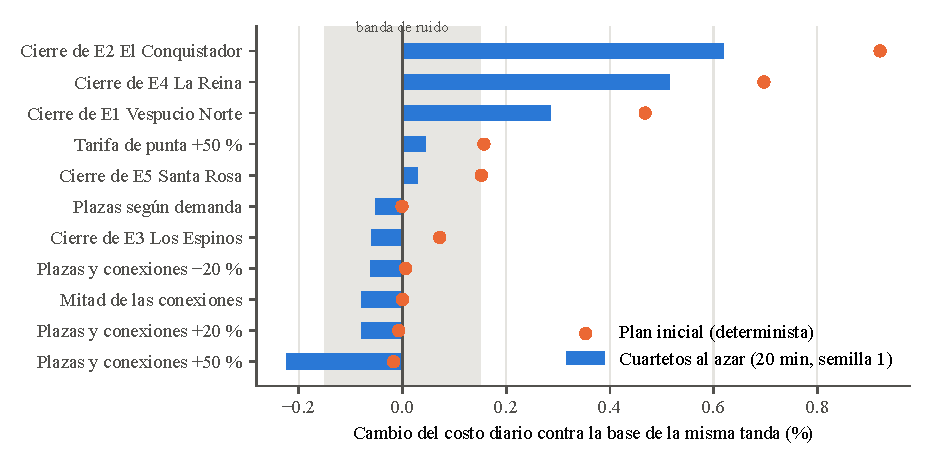
\includegraphics[width=\textwidth]{figures/sensibilidad.pdf}
\caption{Cambio del costo diario en cada escenario de capacidad y tarifa. La franja gris es el ruido entre semillas de la búsqueda.}
\label{fig:sensibilidad}
\end{figure}

Las plazas y las conexiones no limitan la flota en el día aislado, entre 20\,\% menos y 50\,\% más. Con la mitad de las conexiones el plan inicial sale idéntico, lo que coincide con que durante el día se usa como máximo cerca de un quinto de ellas (sección~\ref{sec:uso-e}). Con 50\,\% más de plazas la flota de cuartetos cambia en \SensBusesPlazasMasCincuenta{} buses, pero eso está en el borde del ruido y el plan inicial no se mueve, así que para afirmarlo harían falta más semillas. La tarifa de punta más cara sube el costo del plan inicial en USD~\SensUsdInicialTarifaPunta{} al día (\SensCostoInicialTarifaPunta\,\%), y con cuartetos la diferencia queda dentro del ruido, porque la energía es una fracción mínima del costo.

\section{El bus}
\label{sec:sens-bus}

El bus mismo pesa mucho más que la infraestructura (Tabla~\ref{tab:fisicos}). Con una batería de 250~kWh la flota cambia en \FisDeltaBusesBatDoscientosCincuenta\,\%, y con 20\,\% más de consumo, en \FisDeltaBusesConsumoVeinte\,\%. Con menos autonomía cada bus alcanza a hacer menos corridas antes de tener que cargar, y la carga pasa a ocupar huecos que antes servían para encadenar. La pregunta relevante, sin embargo, es si el ahorro frente al caso base se mantiene, y para responderla el caso base se corrió con la misma batería y el mismo consumo de cada escenario. El caso base también crece, y el ahorro de costo del método queda entre \FisAhorroMin{} y \FisAhorroMax\,\%, prácticamente igual al de la base de la tanda.

\begin{table}[htbp]
\centering
\caption{Sensibilidad a la batería y al consumo, día laboral. Cuartetos al azar con 20 minutos y una semilla; el caso base usa la misma batería y el mismo consumo de cada escenario.}
\label{tab:fisicos}
\footnotesize
\resizebox{\textwidth}{!}{%
\begin{tabular}{@{}lrrrrrrr@{}}
\toprule
 & Batería & Consumo & Buses & Buses & $\Delta$ buses & $\Delta$ costo & Ahorro vs \\
Escenario & (kWh) & (kWh/km) & caso base & plan & plan (\%) & plan (\%) & caso base (\%) \\
\midrule
\tabla{fisicos}
\bottomrule
\end{tabular}}
\fuente{\texttt{09-entrega3/sensibilidad/resultados/fisicos\_417\_L.csv} y \texttt{ahorro\_fisicos.csv}.}
\end{table}

\section{Precios}
\label{sec:sens-precios}

Con el costo por bus o por kilómetro un 20\,\% más alto o más bajo, el ahorro del día laboral queda entre \CostosAhorroMin{} y \CostosAhorroMax\,\% (Tabla~\ref{tab:costos}). Encarecer los buses aumenta un poco el ahorro, porque el método ahorra sobre todo buses, y encarecer los kilómetros lo reduce un poco. Cobrar la espera entre corridas, a USD~\CostoEsperaMinuto{} por minuto, suma cerca del \PctEspera\,\% al costo de ambos planes y deja el ahorro en \AhorroConEspera\,\%. Estos escenarios no se reoptimizaron, de modo que muestran el ahorro de los mismos planes con otros precios.

\begin{table}[htbp]
\centering
\caption{Ahorro de costo del plan frente al caso base con otros precios, sin volver a optimizar (\%).}
\label{tab:costos}
\small
\begin{tabular}{@{}lrrr@{}}
\toprule
Escenario & Laboral & Sábado & Domingo \\
\midrule
\tabla{costos}
\bottomrule
\end{tabular}
\fuente{\texttt{09-entrega3/sensibilidad/resultados/costos\_evaluados.csv} y \texttt{09-entrega3/kpi/resultados/costo\_espera.csv}.}
\end{table}

\section{Incertidumbre en los tiempos de viaje}
\label{sec:incertidumbre}

Los planes se construyen con los tiempos nominales del GTFS, pero en la operación hay congestión. Para medir qué tan frágil es cada plan se simuló su día laboral con tiempos aleatorios, multiplicando la duración de cada corrida y de cada traslado por un factor lognormal de media uno, con coeficientes de variación de 10, 20 y 30\,\% y \ReplicasAtrasos{} réplicas por nivel, usando los mismos números aleatorios para ambos planes. En la simulación un bus nunca sale antes de su horario, de modo que si llega tarde el atraso se arrastra, y el cargador queda reservado hasta la hora programada, así que un bus que llega tarde carga menos. No hay despachadores ni buses de reserva.

\begin{table}[htbp]
\centering
\caption{Simulación de atrasos en el día laboral, promedio de \ReplicasAtrasos{} réplicas.}
\label{tab:atrasos}
\footnotesize
\begin{tabular}{@{}rrrrrrrrr@{}}
\toprule
 & \multicolumn{2}{c}{Corridas con más} & \multicolumn{2}{c}{Atraso percentil} & \multicolumn{2}{c}{Buses bajo} & \multicolumn{2}{c}{Buses sin} \\
 & \multicolumn{2}{c}{de 5 min de atraso (\%)} & \multicolumn{2}{c}{95 (min)} & \multicolumn{2}{c}{la reserva} & \multicolumn{2}{c}{energía} \\
\cmidrule(lr){2-3}\cmidrule(lr){4-5}\cmidrule(lr){6-7}\cmidrule(lr){8-9}
Variación (\%) & Base & Plan & Base & Plan & Base & Plan & Base & Plan \\
\midrule
\tabla{atrasos}
\bottomrule
\end{tabular}
\fuente{\texttt{09-entrega3/incertidumbre/resultados/atrasos.csv}.}
\end{table}

El plan es más frágil que el caso base (Tabla~\ref{tab:atrasos} y Figura~\ref{fig:atrasos}). Con una variación de 10\,\%, el \AtrasadasPlanDiez\,\% de sus corridas sale con más de cinco minutos de atraso, contra el \AtrasadasBaseDiez\,\% del caso base, y \BajoReservaPlanDiez{} buses bajan de la reserva, contra \BajoReservaBaseDiez{}. La explicación está en lo que el método optimiza. Usa menos buses, de modo que hay menos tiempo libre entre corridas para absorber atrasos, y carga solo la energía necesaria, de modo que si un atraso acorta una carga el bus termina bajo la reserva. El caso base, que carga siempre al 100\,\%, tiene un colchón de energía que el plan no tiene. Antes de operar el plan hay que darle holgura, con un margen de energía sobre la reserva en el MILP de recargas, tiempo de colchón antes de cada carga o algunos buses de reserva. Esa holgura le restará parte del ahorro, y cuánto queda por medir. La simulación además supone atrasos independientes, cuando en la realidad la congestión afecta a muchas corridas a la vez, así que los resultados reales podrían ser peores.

\begin{figure}[htbp]
\centering
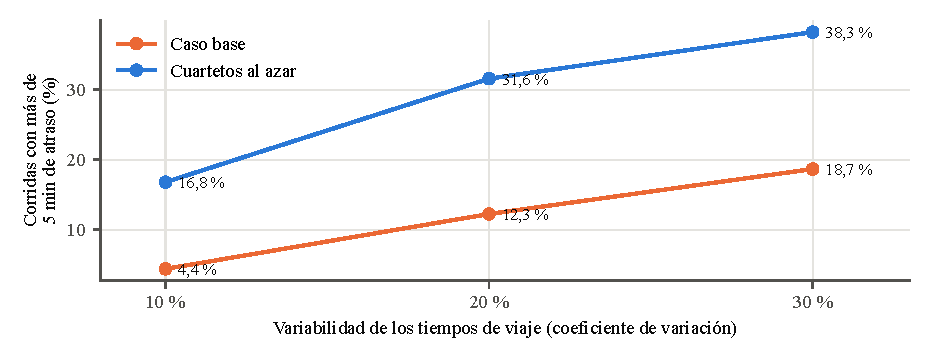
\includegraphics[width=\textwidth]{figures/atrasos.pdf}
\caption{Corridas con más de cinco minutos de atraso según la variabilidad de los tiempos de viaje, día laboral.}
\label{fig:atrasos}
\end{figure}

\section{Repetibilidad del día siguiente}
\label{sec:repetibilidad}

El enunciado fija que todos los buses parten el día con la batería llena, y ambos planes lo cumplen. Pero en la Entrega~2 el equipo docente preguntó cómo se cubre el día siguiente. En el plan los buses terminan el día laboral con \EnergiaFinalPlanLaboral~kWh en promedio, contra \EnergiaFinalBaseLaboral{} en el caso base, porque cargan muy poco durante la operación. Para volver a partir llenos hay que reponer \ReponerMwhLaboral~MWh durante la noche.

Para saber si eso es posible se supuso que cada bus carga en el electroterminal de su sector durante su ventana nocturna, que va de su última llegada a su primera salida del día siguiente, y que todas las conexiones trabajan a \Potencia~kW durante toda la ventana. La Tabla~\ref{tab:repetibilidad} muestra el resultado. En día laboral la ventana mediana dura \VentanaMedianaLaboral{} horas y en ella las \ConexionesTotales{} conexiones alcanzan a entregar solo el \PctCubiertoLaboral\,\% de la energía necesaria. Para reponerla toda harían falta \MwNecesariosLaboral~MW en vez de los \MwInstalados{} instalados, o \ConexionesNecesariasLaboral{} conexiones. El problema es general, aunque desigual. La Reina cubre el menor porcentaje (\ReposPeorPct\,\%) y a Santa Rosa le faltan más conexiones (\ReposMasFaltan), mientras que Vespucio Norte cubre el \ReposMejorPct\,\%. El sábado y el domingo, con menos buses y ventanas más largas, se cubre el \PctCubiertoSabado{} y el \PctCubiertoDomingo\,\%.

\begin{table}[htbp]
\centering
\caption{Recarga nocturna necesaria para repetir el día, por tipo de día.}
\label{tab:repetibilidad}
\footnotesize
\begin{tabular}{@{}lrrrrrrr@{}}
\toprule
 & Energía a & Ventana & \multicolumn{2}{c}{Se alcanza a reponer (\%)} & MW & Conexiones & Conexiones \\
\cmidrule(lr){4-5}
Día & reponer (MWh) & mediana (h) & Plan & Caso base & necesarios & necesarias & faltantes \\
\midrule
\tabla{repetibilidad}
\bottomrule
\end{tabular}
\fuente{\texttt{09-entrega3/kpi/resultados/repetibilidad.csv}. Hay \ConexionesTotales{} conexiones y \MwInstalados~MW instalados.}
\end{table}

El caso base tampoco se repite, ya que en día laboral alcanza a reponer el \PctCubiertoBaseLaboral\,\% y le faltan \ConexionesFaltantesBaseLaboral{} conexiones, de modo que el problema está en la infraestructura frente a una flota eléctrica de este tamaño. El plan sí agrava el problema, porque deja más energía por reponer (\ReponerMwhLaboral{} contra \ReponerBaseMwhLaboral~MWh) y parte de su ahorro en energía corresponde a carga que se traslada a la noche. Si a cada plan se le cobra la energía de esa noche, a la tarifa nocturna y con o sin el costo de sesión, el ahorro del día laboral baja de \BajaCostoLaboral{} a entre \AhorroNocheMinLaboral{} y \AhorroNocheMaxLaboral\,\%, y el semanal de \BajaSemana{} a entre \AhorroNocheMinSemana{} y \AhorroNocheMaxSemana\,\%. Casi todo el ahorro se mantiene porque viene de los buses. Estas cifras son una cota optimista, porque no cuentan el traslado hasta el electroterminal, y \BusesTerminanFueraLaboral{} de los \BusesPlanLaboral{} buses terminan el día en terminales sin cargadores.

\section{Implicancias y robustez de las conclusiones}
\label{sec:implicancias}

La conclusión principal, que el plan cubre el mismo servicio con cerca de 15\,\% menos buses y 14\,\% menos costo, resiste todos los escenarios probados. Ni los precios, ni la capacidad de carga, ni el bus la cambian de signo o de orden de magnitud, y aun cobrando la recarga nocturna el ahorro supera el 12\,\%. Para RED esto tiene tres implicancias prácticas. Ampliar plazas o conexiones no reduce la flota en la operación diurna, de modo que esa inversión solo se justifica por la noche. Los electroterminales que más importan en caso de falla son El Conquistador y La Reina, y conviene asegurar su continuidad de servicio. Y la elección del bus, en batería y consumo, pesa más en la flota que cualquier decisión de infraestructura.

Lo que no resiste igual de bien es la operación con atrasos. El plan funciona en el modelo, pero en la calle necesita holgura, y esa es la principal condición para implementarlo (capítulo~\ref{ch:piloto}).

\section{Limitaciones}
\label{sec:limitaciones}

El modelo tiene límites que conviene declarar. Trata un día aislado y no exige terminar con energía, lo que se compensa solo en parte con el análisis de repetibilidad. Supone carga lineal, cuando las baterías reales cargan más lento cerca del 100\,\%, aunque el plan carga poco y rara vez llega a ese tramo. La velocidad en vacío de \VelocidadVacio~km/h, la potencia y el estado de carga inicial no se variaron. Tampoco se modelan conductores, mantenciones ni la capacidad de los terminales comunes. Los sectores fijos impiden combinar corridas de sectores vecinos, y en la red completa la calidad del plan solo se conoce a través de una cota débil.

\section{Extensiones y mejoras}
\label{sec:extensiones}

El análisis sugiere cinco mejoras. Agregar holgura de energía y de tiempo al MILP de recargas, que es la condición para operar el plan, y modelar la noche exigiendo que la energía final permita repetir el día con la capacidad nocturna de cada electroterminal. Probar un movimiento que traspase recargas entre buses, que es lo que limitó la búsqueda con recarga forzada, y grupos con buses de sectores vecinos. Y agregar capacidad a los terminales comunes y una cota más fuerte para la red, por ejemplo con generación de columnas dentro de un sector.
